\documentclass[10pt]{article}
\setlength\parindent{0pt}
\setlength\parskip{1em}
\usepackage{fullpage}
\usepackage{epsf}
\usepackage{amsmath}
\usepackage{graphicx}
\usepackage{fullpage}
\usepackage{graphicx}

\begin{document}

\begin{center}
{\Large A Guerrilla Guide to Musical Notes and Notation}
\end{center}

Here's a very (very) quick guide to reading music and the way musicians talk about notes.

\section {Notes}

\subsection{The white keys}

Notes are named after letters of the alphabet. The white keys on the piano keyboard are named with letters
A through G; after G, the cycle repeats. (For reasons we will discuss later, we usually start with C, and thus count
C, D, E, F, G, A, B, C, etc.)

One repetition of the cycle is called an ``octave''.



{\bf Exercise: With a partner, go to the piano. One person should play a note repeatedly and say its name; the other should 
play notes upward from that, naming each note in turn, until they reach a note that has the same name. What do you 
notice about the sound?}

\vspace{1in}

{\bf Exercise: One person should play two adjacent notes together -- for instance, A and B. They should then move the 
top note up by one key and repeat -- A and C, A and D, A and E, and so forth. Another person, not looking at the keyboard,
should stop them when they reach the octave: two A's played together. (They should tell this just by hearing.)}

\vspace{1in}


\subsection{The black keys}

Of course, there are some notes on the piano keyboard between these: the black keys. Their names involve the 
words {\it sharp} and {\it flat}. {\it Sharp} means that you shift one key upward; {\it flat} 
means that you shift one key downward.

For instance, the black key between C and D could be named either C-sharp or D-flat; both names refer to the same note
on the piano. $\sharp$ is the symbol for ``sharp'', and $\flat$ is the symbol for ``flat''.

Three questions you should discuss with your neighbors:

\begin{enumerate}
\item What is the other name of the note named G$\sharp$?
\item What is the other name of the note named F$\flat$? (There are occasionally reasons we want to do this!)
\item How many different named notes are there? Don't count duplicates, like C$\sharp$ and D$\flat$.
\end{enumerate}


Musicians use the term ``pitch'' to describe whether a note is high or low, and ``interval'' to 
describe the distance between two notes. You already know the term ``octave''
to the interval between two neighboring notes that share names. Here are some others:

\begin{itemize}
\item {\bf Half step: the smallest interval in Western music; the distance between two adjacent keys (white or black)}
\item Second or ``whole step'': two half steps; the distance from C to D
\item Minor third: three half steps; the distance from C to E$\flat$
\item Major third: four half steps; the distance from C to E
\item Fourth: five half steps; the distance from C to F
\item Tritone: six half steps; the distance from C to F$\sharp$
\item {\bf Fifth: seven half steps; the distance from C to G}
\item Minor sixth: eight half steps
\item Major sixth: nine half steps
\item Minor seventh: ten half steps
\item Major seventh: eleven half steps
\item {\bf Octave: twelve half steps}
\end{itemize}

The ones in boldface are ones you should try to learn quickly; the others you can just reference here.

\section {Reading music}

We notate music on a five-lined system called a {\it staff}. Five lines are always drawn, but you can extend 
the staff by drawing more lines on the top or the bottom, as necessary. Dots indicate which note is to be played,
like this:

\begin{center}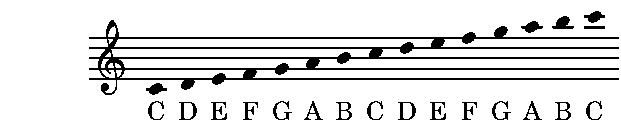
\includegraphics[width=0.6\textwidth]{staff1-crop.pdf}\end{center}

The first note shown here -- one line below the staff -- is called ``middle C''. It has this name because it is a
low but reasonable note for most women to sing, and a high but reasonable note for most men to sing -- right in the 
middle of the piano keyboard.

The funny squiggle at the beginning of this staff is called a ``treble clef''. We can use a different symbol to write
lower notes, called a ``bass clef''; it works the same way, except the symbol is different, and middle C is the line
{\it above} the staff.

Usually music written for instruments with a limited range (like violins, trumpets, or the human voice)
is written on only one staff. Music written for instruments with a very wide range, like the piano, is 
written on two staves on top of each other -- one in bass clef and one in treble clef.

Here, for instance, is a sequence of many of the white keys on a piano, starting two octaves below middle C
and ending two octaves above it. (This, incidentally, is close to the extreme ranges of the human voice, from
low male voices to high female voices.)

\begin{center}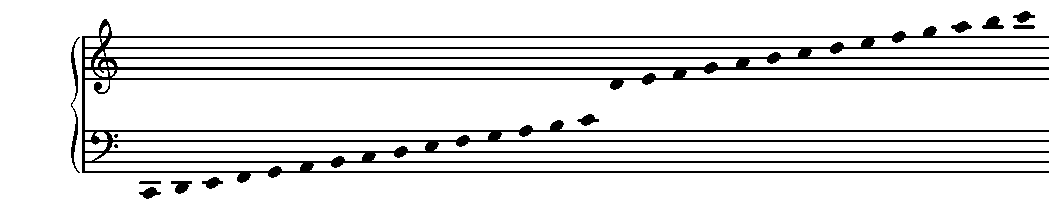
\includegraphics[width=\textwidth]{staff2-crop.pdf}\end{center}

Here is a sequence of {\it all} of the keys, white and black, going from one octave below middle C to one 
octave above it. (I wrote all the black keys as sharps, but you could just as easily have written them as flats.)

\begin{center}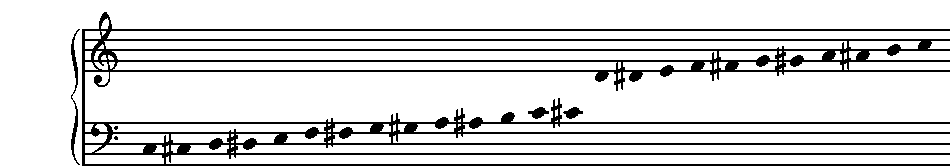
\includegraphics[width=\textwidth]{staff3-crop.pdf}\end{center}



\end{document}


